\documentclass{article}
\usepackage{graphicx}
\usepackage{amssymb}
\usepackage{listings}

\usepackage{color}
\definecolor{codegrey}{gray}{0.92}

\author{Jason Kraftcheck}
\title{Anatomy of a Mesquite 2.0 Quality Improver}
\date{October 8, 2007}

\begin{document}
\maketitle
\tableofcontents
\listoffigures

\lstset{language=c++,basicstyle=\small,showstringspaces=false,backgroundcolor=\color{codegrey}}


\newenvironment{smallmargins}{\addtolength{\hoffset}{-1.0in}\addtolength{\textwidth}{2.0in} }{}

\section{Introduction}

\subsection{Intent}

After the Mesquite 1.1 release and before the release of Mesquite version 2.0 (approx. 2006/2007 fiscal year), a variety of enhancements were made to the Mesquite solver design.  These include:
\begin{itemize}
\item Replacing the element-based and vertex-based quality metric dichotomy with the ability to evaluate quality metrics at any local mesh feature.
\item The introduction of Jacobian-matrix-based target metrics and the evaluation of those metrics at a variety of sample points within a mesh element.
\item Block coordinate descent solvers.
\item Initial work towards smoothing of quadratic finite elements.  
\end{itemize}

The intent of this document is to describe the current design and API for the portions of Mesquite affected by the above changes.  It is the intent of the
author that this document serve both as a description of the design changes
for current developers (both Mesquite developers and those developers using Mesquite in other applications) and as documentation for the discussed portions of Mesquite for future developers.

\subsection{Organization}

A Mesquite quality improver is assembled from instances of the C++ classes representing various components, such as objectve function templates and quality metrics..  Examples of components in Mesquite include the \texttt{FeasibleNewton} solver, the \texttt{JacobianMetric}, and the \texttt{PMeanPTemplate}.  This document is organized beginning with the top-most component, the quality improver, followed by the components required by the quality improver, followed by the subcomponents of those components, and so on.

This document also contains several subsections titled \emph{Future Work}.  These sections are the musings of the author and should not be interpreted as a formal or official plan for future Mesquite changes.   


\subsection{UML}

\begin{figure}[htb]
\begin{center}
\includegraphics[width=3.5in]{fig/UML_class_key}
\caption{UML class diagram elements and coloring scheme.\label{fig:UML}}
\end{center}
\end{figure}

UML diagrams are used throughout this document.  The UML action diagrams should be self-evident even for those not familiar with UML.  However, the UML class diagrams may not be as self-explanatory.  Figure \ref{fig:UML} shows the subset of UML class diagram notation used and in this document.

\begin{figure}[htb]
\begin{center}
\includegraphics[width=\textwidth]{fig/uml-example}
\caption{UML Example\label{fig:UML-Example}}
\end{center}
\end{figure}

The "has-a" relationship, shown with an open-headed arrow in UML diagrams, indicates a loose single-directional association between two objects, typcially implemented by one object having a pointer to another.  For Mesquite components, this relation usually indicates an association a developer must create during component construction.  Strong associations such as aggregation and composition are not shown in the diagrams in this document.  The "derived" or "implements" relationship, shown with an triangle arrow head in UML diagrams, is implemented using class inheritance in C++.  The class at the base of the arrow is derived from the class at the head of the arrow.  In the context of assembling Mesquite solvers, the base class is often a type of class that may be required by some other component and the derived class is one of several instances of that type that can be used to fulfill the requirement.  

Consider the simple example in Figure \ref{fig:UML-Example}.  All implementations of the \texttt{ObjectiveFunctionTemplate} abstract class, such as \texttt{LPtoPTemplate}, require an instance of a \texttt{QualityMetric}.  This is indicated by the black arrow from \texttt{ObjectiveFunctionTemplate} to \texttt{QualityMetric}.  To create an instance of \texttt{LPtoPTemplate} for use in a solver, one would first have to create a \texttt{QualityMetric} instance.  However, as indicated by the italics in the class name ``QualityMetric'' in the diagram, \texttt{QualityMetric} is an abstract class or interface.  One must create an instance of a class that implements the \texttt{QualityMetric} interface.  Examples of such classes in Figure \ref{fig:UML-Example} are \texttt{IdealWeightInverseMeanRatio} and \texttt{ConditionNumberQualityMetric}.  These are concrete classes (the names are not italicized), so instances of them can be created.  The path of red triangle-headed arrows from each of these classes to \texttt{QualityMetric} indicate that both classes provide the \texttt{QualityMetric} interface.  In summary, one can conclude from Figure \ref{fig:UML-Example} that a quality metric such as   \texttt{IdealWeightInverseMeanRatio} or \texttt{ConditionNumberQualityMetric} must be created and used in the creation of a \texttt{LPtoPTemplate} instance.


\subsection{\texttt{MsqError}}

Almost every function in the Mesquite API accepts an instance of the \texttt{MsqError} class and uses that instance to flag the occurance of any errors.  For brevity, this argument is not shown or discussed for any function in the API.  The reader may assume an implicit final argument of type \texttt{MsqError\&} for almost every function shown or discussed in this document, the exceptions being those functions that cannot fail.

The \texttt{MsqError} class can be treated as a Boolean, where a true state indicates an error.  It can also be sent to a C++ output stream to print the error code, error message, and call stack (trace of nested function calls beginning with the topmost API call down to the function at which the error occured.)  An application will typically use an \texttt{MsqError} as follows:
\begin{lstlisting}
if (err) {
  std::cout << err << std::endl;
  return FAILURE;
}
\end{lstlisting}
The \texttt{MsqError} class also provides functions to progamatically extract data from such as the error message, error code, and call stack lines.

Mesquite also provides several macros to assist developers in using the \texttt{MsqError} class within Mesquite.  The \texttt{MSQ\_SETERR} macro is used to flag an initial error condition.  The following examples show typical uses of this macro:
\begin{lstlisting}
  // literal error message and error code
MSQ_SETERR(err)( "My error message", MsqError::UNKNOWN_ERROR );
  // error code and printf-style formatted error message
MSQ_SETERR(err)( MsqError::INVALID_ARG, "Argument 'foo' = %d", foo );
  // error code and default message for that error code
MSQ_SETERR(err)( MsqError::OUT_OF_MEMORY );
\end{lstlisting}

The \texttt{MSQ\_CHKERR} macro evalutes to true if an error has been flagged, and false otherwise.  Further, if an error has been flagged, it appends the location of the \texttt{MSQ\_CHKERR} invokation to the call stack maintained in the \texttt{MsqError} instance.  This is the mechanism by which Mesquite generates the call-stack data.  The following is an example of how this macro is typically used:
\begin{lstlisting}
  if (MSQ_CHKERR(err))
    return FAILURE;
\end{lstlisting}
The macro may also seen used similar to the following example:
\begin{lstlisting}
  return !MSQ_CHKERR(err) && result_bool;
\end{lstlisting}
This statement will result in a return value of \texttt{false} if either an error has been flaged or \texttt{result\_bool} is false.  The order of the tests is important in this example.  The \texttt{MSQ\_CHKERR} macro must occur first so that the call stack is updated, regardless of the value of \texttt{result\_bool}.

\texttt{MSQ\_ERRRTN} and \texttt{MSQ\_ERRZERO}  are convenience macros for developers. They are defined as follows:
\begin{lstlisting}
 #define MSQ_ERRRTN(ERR)  if (MSQ_CHKERR(ERR)) return
 #define MSQ_ERRZERO(ERR) if (MSQ_CHKERR(ERR)) return 0
\end{lstlisting}

\section{Mesh Quality Improvers}

\subsection{Overview}

\begin{figure}[htb]
\includegraphics[width=\textwidth]{fig/quality-improvers-class}
\caption{QualityImprover class diagram.\label{fig:qual-improv-class}}
\end{figure}

All quality improvers in the current Mesquite implementation are subclasses of the \texttt{VertexMover} class.  That is, all quality improvers work by optimizing mesh vertex locations.  They do not make changes to the mesh topology.

\subsection{Patches and the Optimization Loop}

\subsubsection{Patches}

\begin{figure}[htb]
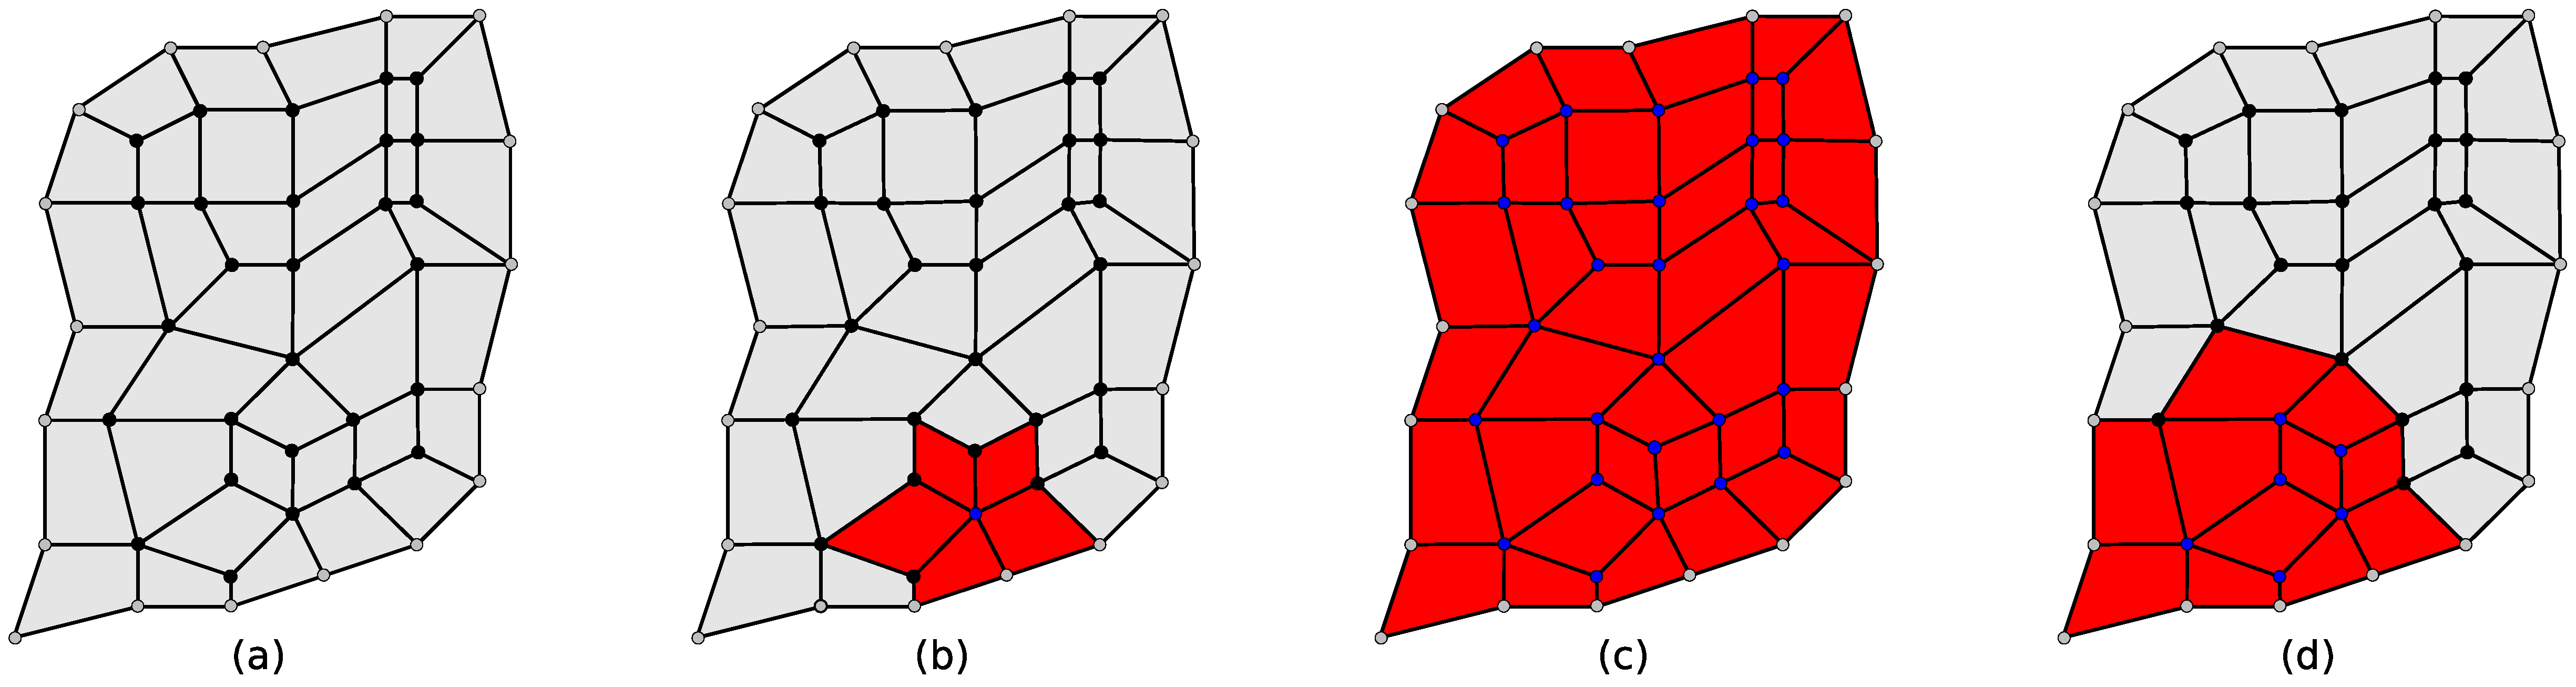
\includegraphics[width=\textwidth]{fig/patches-horiz}
\caption{Miscellaneous patch configurations.\label{fig:patch-types}}
\end{figure}

Optimization of mesh in Mesquite is performed on \emph{patches}.  Given a mesh defined by a set of vertices $V$ and elements $E$, a patch is composed of an arbitrary $W \subset V$,  $F={f \in E, Cl(f) \cup W \ne \emptyset}$.  That is, a patch is defined to be some subset of the vertices to optimize and the elements for which the quality is affected by the position of these verices.  In containing elements, the patch implicitly contains all vertices in the closure of those elements.  Any such implicit vertices that are not also in $W$ ($x \in Cl(E), x \notin W$) are referred to as \emph{fixed} (or less accurately as \emph{boundary}) vertices.  This property should not be confused with the global \emph{fixed} property of vertices $v \in V$.  The latter is an input constraint on the mesh, while the former is a property of the temporary patch data structure, not the actual subset of the mesh represented by the patch.   Patches may overlap, may be disjoint, etc.  

Vertices are marked as fixed in a patch because the positions of those vertices will not be optimized as part of the optimization of the current patch.  Any vertex that is marked as fixed in the input mesh will always be marked as fixed in any patch it occurs in because the coordinates of such a vertex are by definition never optimized.  A vertex may also be marked as fixed in a patch for other reasons, for exaple if it is not in the set of vertices to optimize with the patch but is in the closure of the elements adjacent to said vertices.  The \emph{fixed} state of a vertex in a patch is a property of the patch.  Such a vertex may not be fixed in other patches, and will not be fixed in at least one other patch unless it is marked as fixed by the application as part of the input mesh.  Global patches are the only case where the fixed state in the patch is the same as the fixed state in the input mesh:  all non-fixed vertices in the input mesh are not marked as fixed in a global patch.

Figure \ref{fig:patch-types} illustrates different patch determination schemes.  The left-most mesh (a) is an input mesh supplied by the application, with the fixed vertices colored in grey and the free vertices in black. A single-vertex patch in the same mesh is shown in (b), with the patch elements in red and the free patch vertex in blue.   A global patch is shown in (c) and an appliciation-defined patch in (d).

\subsubsection{Optimization Loop}

\begin{figure}[htb]
\begin{center}
\includegraphics[width=4in]{fig/solver-flow-simple_compact}
\caption{Simplified logical flow of solver.\label{fig:solver-flow}}
\end{center}
\end{figure}

Optimization is subdivided into an outer and an inner loop.  The inner loop is an iterative improvement of the mesh in a patch.  The outer loop is an iteration over all of the patches in the mesh.  Figure \ref{fig:solver-flow} is a simplified UML action diagram for the optimization loop.  

For a simple Laplacian smoother, the patch is always a single free vertex and its adjacent elements.  The inner loop is a single iteration to update the location of that vertex.  The outer loop is a repeated iteration over each vertex in the mesh.

If a patch containing the entire mesh is used, an optimization is said to be a \emph{global} solution.  In such a configuration, all optimization is done in the inner loop.  The outer loop may be considered a single iteration over the set of one patch.

\subsubsection{Solvers}

Many of the quality improvers in Mesquite work by minimizing the value of an objective function (see Section \ref{sec:ObjectiveFunction}), where the objective function is a function of the mesh vertex coordinates.   The term \emph{solver} is often used to refer to the portion of the code in the concrete subclass of \texttt{VertexMover} that implements the inner loop of the optimization for quality improvers that optimize an explicit objective-function based (the code that implements the function-minimization algorithm.)  

The \texttt{FeasibleNewton} and \texttt{ConjugateGradient} implementations are examples of quality improvers that contain solvers.

\subsubsection{PatchSetUser and PatchSet}

A \texttt{PatchSetUser} is an optimizer for which the application may specify how the mesh is decomposed into patches.  \texttt{PatchSetUser} provides two pre-defined patch schemes.  The \texttt{use\_global\_patch()} method will result in a single patch containing the entire mesh.  The \texttt{use\_element\_on\_vertex\_patch()} method will result in a patch for every free vertex in the mesh, containing only the free vertex and its adjacent elements.  An alternate scheme for subdividing the mesh into patches may be specified by providing a custom implementation of the \texttt{PatchSet} interface.

The \texttt{PatchSet} interface defines two methods: \texttt{get\_patch\_handles} and \texttt{get\_patch}.  The \texttt{get\_patch\_handles} method returns a list of handles (or identifiers), one for each potential patch in a mesh.  The \texttt{get\_patch} method returns the free vertices and elements in a patch, given one of the handles passed back from the \texttt{get\_patch\_handles} method.

The \texttt{GlobalPatch} class is the implementation of the \texttt{PatchSet} interface that provides a single patch for the entire mesh.  The \texttt{VertexPatches} class provides the Laplacian-like decomposition of the mesh into a patch for every free vertex.  The \texttt{ElementPatches} class is used internally in places other than the main optimization loop, such as initializing BCD data and in the \texttt{QualityAssessor} class.  It decomposes the mesh into single-element patches with no free vertices.

\subsubsection{Laplacian Quality Improvers}

As shown in Figure \ref{fig:qual-improv-class}, the Laplacian quality improvers do not implement the \texttt{PatchSetUser} interface, and therefore do not allow the selection of a patch definition scheme.  Laplacian smoothers always operate on an element-on-vertex patch with a single free vertex.  

\subsubsection{Nash Game vs. Block Coordinate Descent}

Quality improvers that have an explicit \texttt{ObjectiveFunction} may be used with the block coordinate descent algorithm rather than the default Nash game algorithm if the \texttt{ObjectiveFunction} implementation supports this mode of operation. In a Nash game optimization (the default), the objective function that is optimized by the inner loop is evaluated over only the patch being optimized.  In a block coordinate descent algorithm, the objective function to be optimized in the inner loop is evaluated over the entire mesh.  Only the influence of the current patch vertices on the global objective function is considered during the optimization of each patch.

The selection of Nash vs. BCD algorithms is currently done via the constructors of individual \texttt{QualityImprover} implementations.  In the future this setting will most likely be moved either up to the \texttt{VertexMover} class because it doesn't affect the behavior of the code contained in the concrete solvers or down to the individual \texttt{ObjectiveFunction} implementations, as the core functionality for BCD is provided by individual \texttt{ObjectiveFunction} implementations and it is a characteristic of the individual objective functions that BCD-type algorithms are possible.

\subsubsection{What's New}

Many of the features described in this section are new to the current version of Mesquite.  Mesquite 1.1 was capable of only single-vertex Nash or global optimizations.  It supported neither BCD algorithms nor alternate patch-definition schemes.  

The \texttt{PatchSetUser} and \texttt{PatchSet} classes were added after the 1.1 release.  In Mesquite 1.1, the API for selecting patch type (single-vertex or global) was provided in the \texttt{QualityImprover} interface, allowing nonsensical code such as requesting a global patch for a Laplacian smoother.  The logic that is now contained in \texttt{VertexPatches} and \texttt{GlobalPatch} was interspersed with the \texttt{PatchData} code for retreiving the defined patch from the \texttt{Mesh} instance.

The new \texttt{PatchSet} class also allows for easy reordering of patches during the optimization loop.  As the code now works with an enumerated list of patches, that list can be reordered without impacting other code.

\subsection{TerminationCriterion}

The \texttt{TerminationCriterion} class provides representation of various criteria that may be used to terminate either the inner or outer loop of the quality improvement process.  A separate instance of the \texttt{TerminationCriterion} class is used for each of the inner and outer loops.  Outer termination criteria are not useful for an optimization using a global patch.  Similarly, inner termination criteria are useless for Laplacian smoothing.  The termination criterion used for these cases is an iteration count of one.  In the future, Mesquite may be further re-factored to remove these sources of potential confusion from the API.

\subsection{Current Issues and Future Work}

There is considerable room for improvement in the current organization of quality improvers.  Issues with the current design include:
\begin{itemize}
\item Laplacian smoothers have a meaningless inner termination criterion.  The user may request an inner termination criteria, but that request is silently ignored.  The inner termination criterion is always effectively a iteration count of one.  However, vertex culling criteria, which are currently associated with the inner \texttt{TerminationCriterion} instance, are applicable to Laplacian smoothers.
\item Global-patch optimizations have a useless and potentially harmful outer termination criterion.  The inner and outer termination criteria are logically equivalent, but iterations in the outer optimization loop are more expensive than inner iterations.
\item Laplacian smoothers have an associated ObjectiveFunction instance that is not (necessarily) optimized by the smoother.
\item For best performance, the evaluation of an outer criterion based on objective function value should depend on the choice between Nash and BCD.  The outer criterion objective function value is assumed to evaluated over the entire active mesh, regardless of the choice between Nash and BCD.  The default method for obtaining the value is to evaluate the objective function over the entire mesh.  This solution works for both Nash and BCD, but is grossly inefficient for BCD, where the value over the entire mesh is already known.  
\item The previous point is \emph{not} true for a termination criterion based on the gradient of the objective function.  The solver does not know the gradient for the objective function over the entire mesh, only the terms of the gradient that are with respect to free vertices in the current patch.
\item For a Nash solution, does it make sense to have an outer termination criterion based on an objective function value for the entire mesh?  If so, does it make sense to limit it to the same objective function that is evaluated over the patch in the inner loop?  Pat: ``Termination criterion for Nash should not include a global OF value, but only the value of the OF on the patch.''
\item If inner and outer termination criteria are separated, the implementation may be inefficient.  However, the different termination criteria groups are logically associated and used by different objects.  Laplacian and global optimizations have only one: either inner or outer.  Other optimizations have two, but the outer is used by the \texttt{VertexMover} class while the inner is used by the solver (e.g. \texttt{FeasibleNewton}.)
\item The LaplacianSmoother class should be generalized as a RelaxationSmoother,
allowing for other relaxation schemes depending on metric values or other criteria.  
\end{itemize}


\section{ObjectiveFunction}

\label{sec:ObjectiveFunction}

\begin{figure}[htb]
\begin{center}
\includegraphics[width=\textwidth]{fig/objective-function-class}
\caption{\texttt{ObjectiveFunction} class diagram.\label{fig:objfunc-class}}
\end{center}
\end{figure}

An objective function is a scalar function of all the vertex coordinates in the active mesh.  The mesh vertex locations are optimized so as to minimize the objective function value.  

The objective functions implemented in Mesquite can be divided into two general categories: template objective functions and composite objective functions.  Template objective functions have an associated \texttt{QualityMetric} instance and typically implement some kind of averaging scheme.  Composite objective functions modify the values of one or two other objective functions, such as scaling the value or summing two values.

Most solvers in Mesquite also require the gradient of the objective function (the partial derivatives of the objective function with respect to the coordinate values of the free vertices in the patch.)  

\label{sec:Hessian} Some quality improvers (currently \texttt{FeasibleNewton}) need to know the Hessian (second partial derivatives) of the objective function.  Only an \texttt{ObjectiveFunction} implementation capable of providing Hessian data may be used with such a solver.  Mesquite provides numerical approximation of objective function gradient values, and of quality metric gradient and Hessian values, but not objective function Hessian values.  Further, Mesquite is capable of working only with Hessians of objective functions that have sparse Hessian matrices.  The Hessian matrix may only contain non-zero terms for vertex pairs that share at least one element.  This limitation is explicit in the implementation of the \texttt{MsqHessian} class, and is implicit in other areas of the code (such as portions of the \texttt{ObjectiveFunction} interface relating to use in a BCD algorithm.)  Some \texttt{ObjectiveFunction} implementations such as \texttt{CompositeOFMultiply} (the product of two other objective function values) and \texttt{StdDevTemplate} have a dense Hessian and therefore cannot be used with solvers requiring a Hessian.

\subsection{Objective Function Support for Block Coordinate Descent}

The \texttt{enum EvalType} was added to allow \texttt{ObjectiveFunction} implementations to support block coordinate descent algorithms efficiently.  Many objective function templates perform averaging of quality metric values.  These objective functions can be calculated as a running total for the working mesh.  This running total cane be updated for changes to the local patch without needing to recalculate quality metric values for other parts of the mesh.  Consider the example of an objective function that is the algebraic mean of an element quality metric $\mu(v \in Cl(e_i))$:
\begin{displaymath}
M = \{ e_1 \cdots e_n \}
\end{displaymath}
\begin{displaymath}
f(M) = \frac{1}{n}\sum_{i=1}^{n}\mu(v \in Cl(e_i))
\end{displaymath}
which can be rewritten as:
\begin{displaymath}
f(M) = \frac{1}{n}g(M)
\end{displaymath}
\begin{displaymath}
g(M) = \sum_{i=1}^{n}\mu(v \in Cl(e_i))
\end{displaymath}
The values of $n$ and $g(M_0)$ can be evaluated by making a single pass over all the elements of the mesh before the optimization begins.  The value of $n$ remains constant for the duration of the optimization (Mesquite does not modify the mesh topology).  Given some patch of the mesh: $P \subset M$, $g(M)$ can be updated for changes $P$ with the rather simple arithmetic:
\begin{displaymath}
g(M) = g(M_0) - g(P_0) + g(P)
\end{displaymath}
That is, the value of $g(P_0)$ is calculated at the beginning of the inner optimizer loop.  The updated value of $g$ (and therefore $f$) can then be calculated for a modified version of the patch by calculating $g(P)$ only.


\subsubsection{Objective Function Derivatives for Block Coordinate Descent}

\texttt{ObjectiveFunction} implementations supporting BCD algorithms are also expected to provide gradient and possibly Hessian data.  In a BCD algorithm, the implementation is expected to supply only the terms of the gradient that are with respect to the free vertices in the current patch.  Similarly, only the Hessian terms that are with respect to only free vertices in the current patch need be provided.  

Given that a patch is guaranteed to contain all elements adjacent to the free vertices (in any context where the gradient or Hessian is required), it is assumed that any objective function capable of meeting the sparseness requirement for the Hessian described in Section \ref{sec:Hessian} will be able to provide gradient and Hessian values for a patch in a BCD context without needing to know any data other than the contents of the current patch and the scalar objective function value for the entire mesh.

Continuing with the algebraic mean example from above:
\begin{displaymath} 
\nabla f = \frac{1}{n} \nabla g
\end{displaymath}
\begin{displaymath}
\mathcal{H} f = \frac{1}{n} \mathcal{H} g
\end{displaymath}
\begin{displaymath}
\nabla g = \sum_{i=1}^{n} \nabla \mu(v \in Cl(e_i))
\end{displaymath}
\begin{displaymath}
\mathcal{H} g = \sum_{i=1}^{n} \mathcal{H} \mu(v \in Cl(e_i))
\end{displaymath}

$\nabla g$ is simply the sum of the $n$ quality metric gradient vectors, one for each element in the mesh.  As the quality metric is, by definition of an element metric, a function only of the vertices of one element the terms of the quality metric gradient containing partial derivatives with respect to the coordinates of any vertex not in the element must be zero.  Therefore the terms of $\nabla g$ that correspond to the partial derivatives of any vertex $v_i$ are zero for any quality metric evaluation over an element not adjacent to $v_i$.  Conversely, the portion of $\nabla g$ corresponding to $v_i$ is a function of only the quality of the elements adjacent to $v_i$.  As the local patch is guaranteed to contain all elements adjacent to $v_i$ if the gradient terms for $v_i$ are requested, it is possible to compute the portion of $\nabla G$ corresponding to the free vertices in the patch without any data other than the patch contents.  The same simple reasoning applies equally for the Hessian of the algebraic mean template.

\subsection{Objective Function Implementations}
\label{sec:objfunc_impl}

The \texttt{ObjectiveFunctionTemplate} is a base class for those objective function implementations that are some kind of average of quality metric values.  The \texttt{ObjectiveFunctionTemplate} class provides the API for associating a \texttt{QualityMetric} with an objective function and it provides a common implementation for initializing coordinate descent optimizations.

Existing template-type objective functions from version 1.1 of Mesquite have been updated for the new interface.  These include: \texttt{LPtoPTemplate}, \texttt{LInfTemplate}, and \texttt{MaxTemplate}.  Of these three, support for coordinate descent optimizations was added to \texttt{LPtoPTempalte} only.

The new objective functions \texttt{PMeanPTemplate}, \texttt{StdDevTemplate}, and \texttt{VarianceTemplate} have also been added.  All three of these objective function templates support block coordinate descent optimization.   

The composite objective functions modify one or two existing objective functions (e.g. adding two together).  All composite \texttt{ObjectiveFunction}s support analytical gradients and coordinate descent optimization if the underlying \texttt{ObjectiveFunction}s do.  Similarly, all except \texttt{CompositeOFMultiply} support analytical Hessians as long as their underlying \texttt{ObjectiveFunction}s do.  \texttt{CompositeOFMultiply} does not have a suitably sparse Hessian (see Section \ref{sec:Hessian}).

\subsection{What's New}

Since Mesquite 1.1, the \texttt{ObjectiveFunction} interface has been re-written to support block coordinate descent optimization.  All \texttt{ObjectiveFunction} implementations have been updated for the interface change and all except min/max-type objective function implementations have been updated to support block coordinate descent optimization.  Appendix \ref{sec:ofiface} contains more detail on the interface-level changes to the \texttt{ObjectveFunction} class.

Mesquite 1.1 did not support analytical gradient or Hessian optimization in composite objective functions.  This missing functionality has been added.  All \texttt{ObjectiveFunction} implementations have also been updated for changes to the \texttt{QualityMetric} interface (see below.)

The \texttt{PMeanPTemplate}, \texttt{StdDevTemplate} and \texttt{VarianceTemplate} classes have been added subsequent to the Mesquite 1.1 release.


\section{QualityMetric}

The \texttt{QualityMetric} class provides a measure of the quality at a local mesh feature, such as an element or a vertex.  Figure \ref{fig:qmclass} is the class diagram for all quality metrics (except the legacy DFT metrics discussed in Section \ref{sec:DFT}) in Mesquite.  The basic interface for the \texttt{QualityMetric} class is shown in Figure \ref{fig:qmiface}. 


\begin{figure}[p]
\begin{smallmargins}
\includegraphics[angle=270,width=6in]{fig/quality-metric-class-all}
\caption{\texttt{QualityMetric} Classes.\label{fig:qmclass}}
\end{smallmargins}
\end{figure}


\subsection{Averaging Metric Values}

\label{sec:qmaverage}

There are two classes in Mesquite defining interfaces for averaging quality metric values: \texttt{AveragingQM} and \texttt{PMeanPMetric}.  These classes are typically used for averaging corner or sample-based quality metric values at a vertex or over an element.  Neither is a subclass of \texttt{QualityMetric}.  Both are expected to be used as a base class for quality metric implementations that inherit the \texttt{QualityMetric} interface separately.  These utility classes provide the user API for selecting the averaging scheme.  They also provide utility methods for averaging metric values, gradients, and Hessians for use by the subclass implementing the \texttt{QualityMetric} interface.

The \texttt{AveragingQM} class provides the same enumeration of averaging schemes that was defined in \texttt{QualityMetric} in Mesquite 1.1.  The user selects from a list of averaging schemes such as \texttt{LINEAR}, \texttt{RMS}, \texttt{SUM\_SQUARED}, \texttt{MAXIMUM}, \texttt{MAX\_MINUS\_MIN}, etc.  Many metrics that are internally corner-based for non-simplex elements implement this interface, converting such cases to element-based metrics.  Most element-based quality metrics from Mesquite 1.1 are examples of this type of metric.  Some metrics that are internally corner-based or edge-based implement this interface to provide a vertex-based metric by averaging the values around a vertex.  Most of the vertex-based quality metrics from Mesquite 1.1 are examples of this type of metric.  See the \texttt{QualityMetric} class diagram (Figure \ref{fig:qmclass}) for a list of metrics implementing this interface.

The \texttt{PMeanPMetric} accepts a single parameter: the P-value.  The result is a power-mean of a set of values raised to the P power: $\frac{1}{n}\sum_{i=0}^{n-1}\mu_i^p$.  As shown in Figure \ref{fig:qmclass}, this class serves as a base class for two subclasses: \texttt{ElementPMeanP} and \texttt{VertexPMeanP}.  These classes require an instance of a concrete sample-based quality metric to function.  They work as a type of composite metric, converting the sample-based metric to an element-based or vertex-based metric, respectively, by averaging the metric values for the appropriate sample points. 

The \texttt{ElementMaxQM} and \texttt{VertexMaxQM} are similar to the \texttt{ElementPMeanP} and \texttt{VertexPMeanP} in that they convert sample-based metrics to element-based or vertex-based metrics.  Unlike the \texttt{*PMeanP} metrics, these metrics return the maximum metric value for the entity.  

\subsection{Common Evaluation Points}

The three classes: \texttt{ElementQM}, \texttt{VertexQM} and \texttt{ElemSampleQM} provide common functionality for quality metrics evaluated at the respective entity types.  \texttt{ElemSampleQM} also extends the \texttt{QualityMetric} with functions to provide additional information required by classes such as \texttt{ElementPMeanP} (see Section \ref{sec:qmaverage}).  It is not necessary for a metric of a conceptual type to be a subclass of any of these existing classes (with the exception of the case where one wishes to use a sample-based metric with one of the averaging classes described in Section \ref{sec:qmaverage}).  The \texttt{ElementQM} and \texttt{VertexQM} classes provide utility methods for generating evaluation lists and other functionality that is common for all subclasses.

\subsection{Composite QualityMetrics}

The set of \texttt{QualityMetric} implementations that provide a modification of the output of one or more other \texttt{QualityMetric} implementations are referred to as \emph{composite} quality metrics.  Examples of composite metrics include:
\begin{description}
\item{\texttt{ScalarAddQualityMetric}}: Offset the value of a metric by a constant amount.
\item{\texttt{ScalarMultiplyQualityMetric}}: Scale the value of a metric by a constant amount.
\item{\texttt{PowerQualityMetric}}: Raise the value of a metric to a constant power.
\item{\texttt{AddQualityMetric}}: Add two quality metric values together.
\item{\texttt{MultiplyQualityMetric}}: Multiply the values of two quality metrics.
\end{description}

The composite metrics that operate on multiple underling \texttt{QualityMetric} instances (\texttt{AddQualityMetric} and \texttt{MultiplyQualityMetric}) require metrics that evaluate on the same type of entity.  For example, if one metric is vertex-based, the other should be also.  Otherwise the code has no mechanism to determine which pairs of metric values should be combined.  This is typically enforced by requiring the \texttt{get\_metric\_type} method return the same value and that the \texttt{get\_evaluations} method returns the same list of values for the same patch (see Appendix \ref{sec:qmiface} for an explanation of the \texttt{QualityMetric} interface.)   The mechanism for encoding evaluation handles for sample-based metrics was designed such that it is possible to combine an element-based metric with a sample-based metric (Section \ref{sec:sample-metrics} if the sample-based metric is evaluated at only one sample point in each element.  Sample-based metrics may be combined in a composite metric if they evaluate elements at the same set of sample points.

\subsection{Sample-Based Metrics}
\label{sec:sample-metrics}
A sample-based metric is evaluated at one or more logical sample points within each element of the mesh. The sample-based metrics currently provided in Mesquite are \texttt{JacobianMetric}, \texttt{AffineMapMetric}, \texttt{DomainSurfaceOrientation}, \texttt{TargetSurfaceOrientation}, and the legacy DFT metrics (See Section \ref{sec:DFT}). \texttt{AffineMapMetric} exists primarily for research purposes and will not be discussed further.

\begin{figure}[htb]
\begin{center}
\includegraphics[width=\textwidth]{fig/JacobianMetric_class}
\caption{\texttt{JacobianMetric} Class Diagram.\label{fig:JacobianMetric}}
\end{center}
\end{figure}

As shown in Figure \ref{fig:JacobianMetric}, \texttt{JacobianMetric} class combines the functionality of a \texttt{SamplePoints} instance, a \texttt{TargetMetric2D} and/or a \texttt{TargetMetric3D}, a \texttt{TargetCalculator} and a \texttt{WeightCalculator} for an \texttt{ElemSampleQM} (which is a \texttt{QualityMetric}).  This diagram is a subset of the larger \texttt{QualityMetric} class diagram (Figure \ref{fig:qmclass}.).  

The \texttt{TargetMetric2D} and \texttt{TargetMetric3D} classes are metrics that compare a pair of 2x2 or 3x3 matrices, respectively.  For surface elements (e.g. triangles or quadrilaterals), the \texttt{JacobianMetric} class constructs a 2x2 matrix by rotating the 3x2 Jacobian of the element into the plane of the target 3x2 matrix.  The \texttt{TargetCalulator} instance provides the 3x3 and/or 3x2 matrices that the matrix metrics compare to the element Jacobian.  The \texttt{WeightCalculator} provides a scalar weight at each sample point that is multiplied with the value of the target metric to produce the quality metric.

The rotation from 3x2 Jacobian to the 2x2 matrix passed to the \texttt{TargetMetric2D} in \texttt{JacobianMetric} discards 3D orientation data for surface elements.  The \texttt{DomainSurfaceOrientation} and \texttt{TargetSurfaceOrientation} classes provide a means to evaluate the relative 3D orientation of surface elements.  They can be combined with a \texttt{JacobianMetric} using a composite quality metric.  The \texttt{DomainSurfaceOrientation} metric compares the local element normal (as provided by the Jacobian) with the normal of the geometric domain at the point closest to the location of the element sample point.  The \texttt{TargetSurfaceOrientation} compares the normals provided by the 3x2 Jacobian matrix and the 3x2 target matrix.

\subsubsection{\texttt{SamplePoints}}
The \texttt{SamplePoints} class provides a mechanism for an application to specify where in each element the \texttt{JacobianMetric} should be evaluated.  The application may specify any combination of logical sample points: corners, mid-edge, mid-face, and mid-element.  These values may be specified independently for each element topology (triangle, quadrilateral, etc.)  

\begin{figure}[htb]
\begin{center}
\includegraphics[width=0.9\textwidth]{fig/SamplePoints_interface}
\caption{\texttt{SamplePoints} Class.\label{fig:SamplePoints}}
\end{center}
\end{figure}

The interface for the \texttt{SamplePoints} class is shown in Figure \ref{fig:SamplePoints}.  The first constuctor, by default, initializes an empty \texttt{SamplePoints} instance (no sample points selected for any element topology.)  If that constructor is passed a value of \texttt{true}, then it will initialize with the defaults of one sample point at the center of each simplex and sample points at the corners for other element topologies.  The second constructor can be used to select a common set of logical sample points for all element topologies.  

The \texttt{sample\_at} method adds a logical set of points to the sample points for a specific element topology.  The corresponding \texttt{dont\_sample\_at} method removes a set of logical sample points.  The \texttt{will\_sample\_at} can be used to test if a given set of logical sample points will be evaluated for a specific element topology.  Each of these methods accepts two arguments.  The first indicates the element topology (triangle, hexahedron, etc.)  The second argument, \texttt{dimension}, specifies a logical set of sample points by the portion of the element topology that they lie on: 0 for corners, 1 for edges, 2 for mid-face, and 3 for mid-element.  

In Figure \ref{fig:JacobianMetric}, it can be seen that the \texttt{SamplePoints} instance is associated with the subclasses of \texttt{ElemSampleQM}.  It may at first seem that it would be more logical to associate the \texttt{SamplePoints} instance with the \texttt{ElemSampleQM} because all such metrics are evaluated at sample points.  The reason the design is as shown is that the \texttt{SamplePoints} class provides a mechanism for the application to customize which sample points a metric is evaluated at.  Some metrics that are evaluated at element sample points may only allow a pre-defined set of element sample locations for each element topology.  For example, the legacy DFT metrics (not show, see Section \ref{sec:DFT}) always evaluate at element corners.  As another example; it may eventually be desirable to implement many of the existing element-based metrics as sample-based metrics.  These metrics have one evaluation for simplicies and are evaluated at the corners for other element topologies.  In both examples, the metrics are sample-based but neither allow the application to select which sample points.

\subsection{Mapping Functions}

A \texttt{MappingFunctionSet} must also be specified for a Jacobian-based metric to work.  The \texttt{MappingFunctionSet} instance is not associated with any particular metric because a) it is assumed that if there are multiple Jacobian-based metrics in use that they will share a common \texttt{MappingFunctionSet} and b) for the planned handling of higher-order nodes a single definitive \texttt{MappingFunctionSet} must be available to determine the placement of \emph{slave} higher-order nodes.  An instance of a \texttt{MappingFunctionSet} must be passed to the top-level \texttt{InstructionQueue::run\_instructions} method along with the \texttt{Mesh} and \texttt{MeshDomain} instances.

\begin{figure}[htb]
\begin{center}
\includegraphics[width=\textwidth]{fig/MappingFunction}
\caption{\texttt{MappingFunction} interface.\label{fig:MappingFunction}}
\end{center}
\end{figure}

A \texttt{MappingFunctionSet} is a group of \texttt{MappingFunction} instances, one for each element topology.  Each \texttt{MappingFunction} provides methods to query the value and derivatives of the mapping function.  Figure \ref{fig:MappingFunction} shows the interfaces for the \texttt{MappingFunction} and \texttt{MappingFunctionSet} classes.

A mapping function is assumed to be of the form:
\begin{displaymath}
\vec{x}(\vec{\xi})=\sum_{i=1}^n N_i(\vec{\xi})\vec{x_i}
\end{displaymath}
where $\vec{x_i}$ is a point in $\mathbf{R}^3$ (i.e. $x_i,y_i,z_i$), $\vec{\xi_i} = \left\{\begin{array}{c}\xi_i\\ \eta_i\\ \end{array}\right\}$ for surface elements and $\vec{\xi_i} = \left\{\begin{array}{c}\xi_i\\ \eta_i\\ \zeta_i\\ \end{array}\right\}$ for volume elements.  For example,  a linear quadrilateral element will have a mapping function of the form:
\begin{displaymath}
\vec{x}(\xi,\eta)=N_1(\xi,\eta)\vec{x_1}
                      +N_2(\xi,\eta)\vec{x_2}
                      +N_3(\xi,\eta)\vec{x_3}
                      +N_4(\xi,\eta)\vec{x_4}
\end{displaymath}

A single implementation of the mapping function interface may support multiple elements types of the same topology (e.g. both a 8-node hex and a 20-node hex.)  The \texttt{nodebits} argument to each evaluation function in the interface is passed to specify which higher-order nodes are present in the element.  

The \texttt{coefficients\_at\_*} methods return the values of the mapping function coefficients evaluated at different parameter-space coordinates (the value of the $N_i$ terms for different pre-defined values of $\vec{\xi}$.)  These methods are assumed to pass back a coefficient for each vertex in the element, in the canonical order.

The \texttt{derivatives\_at\_*} methods return the partial derivatives of the mapping function coefficients with respect to the parameters.  These values can be used to construct the Jacobian of the mapping function and the derivative of the Jacobian with respect to the vertex coordinates.  See the Doxygen comments for the \texttt{MappingFunction} class for more details.

Mesquite currently provides only one \texttt{MappingFunctionSet} implementation with a complete set of \texttt{MappingFunction} implementations (one for each element topology): \texttt{LinearFunctionSet}.  The \texttt{LinearFunctionSet} provide shape functions constructed for linear elements (elements without higher-order nodes.)  Mesquite also contains the \texttt{QuadLagrangeShape}, \texttt{TetLagrangeShape} and \texttt{TriLagrangeShape} classes.  These classes provide shape functions constructed from Lagrange polynomials.  They support any combination of higher-order nodes (e.g. a quad with a mid-edge node on only one edge.)  This support for degenerate higher-order elements is provided with the intention of allowing \emph{slave} higher-order nodes in elements.  A \emph{slave} node's location is defined by the mapping function, as opposed to defining the mapping function.  It therefore cannot be included in the evaluation of the mapping function.


\subsection{What's New}

The \texttt{QualityMetric} interface has been generalized to allow metric types other than vertex-based and element-based.  All existing quality metrics have been converted to this interface.  This change substantially reduced duplicate code in composite metrics, numerical derivative approximation, objective function templates, etc.

Mesquite 1.1 had the functionality now provided by \texttt{AveragingQM} as part of the \texttt{QualityMetric} interface.  This was moved into a separate interface so that only the metrics that support this API provide it.  The work on consolidating the code for averaging metric values, gradients, and Hessians that was begun before Mesquite 1.1 was completed as a part of this change.  In the future, it may make sense to transition to a scheme similar to the subclasses of \texttt{PMeanPMetric}, where the existing \texttt{AveragingQM} present themselves as corner-based metrics and a separate class is used to average the metric values.  This would eliminate the need for two separate implementations of the condition number metric (\texttt{ConditionNumberQualityMetric} and \texttt{VertexConditionNumberQualityMetric}).

Complete implementations of analytical gradient and Hessian calculations have been added for all composite metrics.  

The \texttt{JacobianMetric} class and all supporting functionality (\texttt{MappingFunction}, \texttt{MappingFunctionSet}, \texttt{TargetMetric2D}, \texttt{TargetMetric3D}, \texttt{TargetCalculator}, \texttt{WeightCalculator},
\texttt{SamplePoints}, etc.) is completely new.  These new capabilities are discussed further in the next section.


\subsection{Future Work}

 \texttt{VertexPMeanP} (Section \ref{sec:qmaverage}) currently averages metric values at corners regardless of the sample points (Section \ref{sec:sample-metrics}) that the metric is to be evaluated at.  This should be corrected such that any sample points that are influenced by the coordinates of the vertex are included in the average.
 
Some performance gain could most likely be achieved by specializing the current simple implementation of the \texttt{VertexPMeanP} metric for more common P values, similar to the \texttt{PMeanPTempalte} (Section \ref{sec:objfunc_impl}.) 
The entire sample-based metric implementation is in a preliminary state.  Large portions of this functionality remain unimplemented:
\begin{itemize}
\item There are no mapping functions for higher-order elements with hexahedral, pyramidal, or prism topologies.
\item The majority of the 3D target metrics have yet to be implemented.
\item None of the target metrics support analytical gradient or Hessian calculations.
\item The \texttt{JacobianMetric} class does not support analytical gradient or Hessian calculations.
\item There is no provision for dealing with the derivatives of targets or weights that are a function of position.
\item No profiling or subsequent optimization has been done for this code.
\end{itemize}

\section{Target and Weight Calculators}

Figure \ref{fig:target-all-classes} is a UML diagram of the classes discussed in this section.  Referring to this figure and Figure \ref{fig:qmclass} may help in understanding how classes discussed in this section fit into the larger Mesquite solver API.

\begin{figure}[ptb]
\begin{center}
\includegraphics[width=\textwidth]{fig/target-all-classes}
\caption{Target-Related and Weight-Related Classes\label{fig:target-all-classes}}
\end{center}
\end{figure}

\subsection{Target Calculators}

\begin{figure}[htb]
\begin{center}
\includegraphics[width=\textwidth]{fig/target-and-weight-interfaces}
\caption{\texttt{TargetCalculator} and \texttt{WeightCalculator} Interfaces.\label{fig:target-iface}}
\end{center}
\end{figure}

A target matrix ($W$) is compared to an active matrix by a target metric.  The active matrix is typically the Jacobian of the element mapping function at a sample point within the element.  For example, the \texttt{JacobianMetric} class compares the Jacobian of the element to a target matrix using a \texttt{TargetMetric3D} or \texttt{TargetMetric2D} instance.  See Section \ref{sec:sample-metrics} for more detail about target metrics and sample-based quality metrics.

The \texttt{TargetCalculator} class defines an interface for obtaining target matrices.  The \texttt{TargetCalculator} is shown in Figure \ref{fig:target-iface} The two primary functions are \texttt{get\_target\_2D} and \texttt{get\_target\_3D}.  Both functions are passed sufficient data to identify a specific sample point on a specific element.  Both functions pass back a target matrix.  For \texttt{get\_target\_2D}, a 3x2 matrix is returned.  This matrix is compared with the 3x2 Jacobian matrix for surface elements.  The \texttt{get\_target\_3D} function returns a 3x3 target for comparison with the Jacobian of volume elements.

The \texttt{surface\_targets\_are\_3D} method in \texttt{TargetCalculator} allows for backwards compatibility with legacy DFT target calculators (see Section \ref{sec:DFT}.)  A return value of \texttt{true} indicates a legacy DFT target calculator, which generates 3x3 targets for surface elements.  Many of the utility classes discussed in this section may also be used with legacy DFT code.

\begin{figure}[htb]
\begin{center}
\includegraphics[width=3in]{fig/concrete-target-calculators}
\caption{\texttt{TargetCalculator} Implementations.\label{fig:target-concrete}}
\end{center}
\end{figure}

Figure \ref{fig:target-concrete} shows the three true target calculators implemented in Mesquite as of this writing (as opposed to utility classes that also implement the \texttt{TargetCalculator} interface.)  Reference meshes and the \texttt{RefMeshTargetCalculator} are discussed in Section \ref{sec:RefMesh}.

The \texttt{IdealTargetCalculator} returns the Jacobian of an ideal element at the sample point corresponding to the logical sample location in the active element.  The default behavior for surface elements is to rotate the ideal element such that the normal of the ideal and active elements are aligned at the logical sample point before calculating the Jacobian of the ideal element.  This behavior can be disabled, resulting in surface targets for ideal elements in the xy-plane.

The \texttt{LVQDTargetCalculator} combines four other target calculators using an LVQD factorization:
\begin{displaymath}
\mathbf{W} = \lambda(\mathbf{W_\lambda}) \times \mathbf{V}(\mathbf{W_V}) \times \mathbf{Q}(\mathbf{W_Q}) \times \mathbf{\Delta}(\mathbf{W_\Delta}) 
\end{displaymath}
The $\lambda$ function returns a the scalar size component of the $\mathbf{W_\lambda}$ term.  The $\mathbf{V}$ function returns the orientation component of the $\mathbf{W_V}$ term.  $\mathbf{Q}(\mathbf{W_Q})$ is the shape component of $\mathbf{W_Q}$.  The $\mathbf{\Delta}$ function returns the aspect ratio component of $\mathbf{W_\Delta}$.  

\subsection{Weight Calculators}

A sample weight is a scalar weight that is multiplied with the result of a \texttt{TargetMetric} or other sample-based quality metric evaluation.  The \texttt{WeightCalculator} class defines an interface for obtaining weights for each sample point in each element over which the metric is evaluated.  The single method defined by \texttt{WeightCalculator} (see Figure \ref{fig:target-iface}) is \texttt{get\_weight}.  The \texttt{get\_weight} method accepts sufficient parameters to identify an element and a sample point in that element.  It returns the corresponding weight.  See Section \ref{sec:sample-metrics} for more detail about how sample weights are used in the Mesquite API.

\begin{figure}[htb]
\begin{center}
\includegraphics[width=3in]{fig/concrete-weight-calculators}
\caption{\texttt{WeightCalculator} Implementations.\label{fig:weight-concrete}}
\end{center}
\end{figure}

Figure \ref{fig:weight-concrete} shows the three concrete \texttt{WeightCalculator} implementations available at the time of this writing.  The \texttt{UnitWeight} is a trivial \texttt{WeightCalculator} returning a constant unit value for all sample locations in all elements.  The \texttt{MetricWeight} and \texttt{InverseMetricWeight} return the value or inverse value, respectively, of a sample-based quality metric value the corresponding location.

\subsection{ReferenceMesh}
\label{sec:RefMesh}

\begin{figure}[htb]
\begin{center}
\includegraphics[width=3in]{fig/ReferenceMeshInterface}
\caption{\texttt{ReferenceMesh Interface}\label{fig:refmeshiface}}
\end{center}
\end{figure}

A reference mesh is another mechanism for generating targets for a \texttt{JacobianMetric}.  A reference mesh is a mesh that is topologically identical to the active mesh, differing only in the location of the vertices.  The target for any element in the active mesh is then the Jacobian of the corresponding element in the reference mesh.  The \texttt{RefMeshTargetCalculator} class provides the implementation of this target calculation scheme.  

\texttt{RefMeshTargetCalculator} uses a class implementing the interface shown in Figure \ref{fig:refmeshiface}.  The single function defined by \texttt{ReferenceMeshInterface} accepts a list of handles for vertices in the \emph{active} mesh and is expected to return the coordinates of the corresponding vertices in the reference mesh.

\begin{figure}[htb]
\begin{center}
\includegraphics[width=\textwidth]{fig/ref-mesh-class}
\caption{Reference Mesh Implementations.\label{fig:refmesh}}
\end{center}
\end{figure}

Figure \ref{fig:refmesh} shows the only current implementation of \texttt{ReferenceMeshInterface}: \texttt{ReferenceMesh}.  The \texttt{ReferenceMesh} class accepts a pointer to a second \texttt{Mesh} instance (the active mesh being the first instance).  It assumes that vertex handles in the active \texttt{Mesh} instance are \texttt{identical} to those in the reference \texttt{Mesh} instance.  This assumption is unlikely to be true in general, however it is true for pairs of VTK files read by \texttt{MeshImpl} for testing purposes and for the \texttt{TagVertexMesh} scenario discussed below.  A more general implementation of \texttt{ReferenceMeshInterface} would require the use of an external API such as the iTaps iRel interface or some application-specific tag convention to provide the mapping between vertices in the active and reference meshes.

The \texttt{TagVertexMesh} class shown in Figure \ref{fig:refmesh} can be used to provide more compact and robust reference mesh data for deforming mesh problems.  The \texttt{TagVertexMesh} class is a general purpose tool that is also useful outside of the context of target calculation (e.g. storing temporary optimization results.)  It provides the \texttt{Mesh} interface using a reference to another instance of the \texttt{Mesh} interface (decorator pattern.)  All calls to the \texttt{Mesh} functions as implemented by the \texttt{TagVertexMesh} class are passed through to the corresponding functions in the underlying \texttt{Mesh} instance, except for those that query or set vertex coordinates.  All vertex coordinate queries are redirected to a tag in the underlying mesh.  This mechanism allows multiple coordinate tripples to be associated with each vertex in the mesh: the true coordinates and any number of alternate values stored in different tags.

To use the \texttt{TagVertexMesh} class to define a reference mesh in a deforming mesh scenario, the first step is to use the utility methods in the class to copy the vertex coordinates in the undeformed mesh to a tag.  After the mesh has been deformed, it then contains the deformed vertex coordinates as the primary coordinates and the original, undeformed coordinates as data stored in a tag.  When optimizing such a mesh, the unadorned \texttt{Mesh} instance is used as the active mesh and the same \texttt{Mesh} instance, wrapped inside a \texttt{TagVertexMesh}, is used as the reference mesh.

\subsection{Caching Targets}

\begin{figure}[htb]
\begin{center}
\includegraphics[width=2.25in]{fig/CachingTargetCalculator}
\caption{\texttt{CachingTargetCalculator}\label{fig:cachetarget}}
\end{center}
\end{figure}

The \texttt{CachingTargetCalculator} class shown in Figure \ref{fig:cachetarget} is a mechanism to cache target matrices on the current \texttt{PatchData}.  It can be used to speed up optimizations when the target matrices are constant for the duration of the optimization.\footnote{The target matrices need only be constant for the duration of the current patch (one iteration of the outer optimization loop).  However, it is unlikely that a practical situation will arise where this condition is met and the targets are not constant for the duration of the optimization.}  Caching of targets is enabled by inserting an instance of the \texttt{CachingTargetCalculator} between the user of the true \texttt{TargetCalculator} (\texttt{JacobianMetric} in Figure \ref{fig:usecachetarget}) and the actual \texttt{TargetCalculator} instance.

\begin{figure}[htb]
\begin{center}
\includegraphics[width=\textwidth]{fig/caching-targets}
\caption{Caching Targets\label{fig:usecachetarget}}
\end{center}
\end{figure}


\subsection{Pre-Calculating Targets and Weights}

\begin{figure}[htb]
\begin{center}
\includegraphics[width=3in]{fig/target-writer-class}
\caption{Classes for Pre-computing Targets and Weights.\label{fig:targetwriter}}
\end{center}
\end{figure}

The classes shown in Figure \ref{fig:targetwriter} provide a mechanism for pre-calculating targets and/or weights and storing them as tag data on a mesh.  The targets are stored by associating either or both a \texttt{TargetCalculator} and a \texttt{WeightCalculator} with an instance of the \texttt{TargetWriter} class.  The \texttt{TargetWriter} class implements the \texttt{Instruction} interface, and therefore is expected to be inserted directly in the \texttt{InstructionQueue}.  

The targets can be calculated at the beginning of an optimization by placing the \texttt{TargetWriter} first in the \texttt{InstructionQueue} instance.  Alternately, the targets can be calculated and stored for later use by running an instruction queue containing only the \texttt{TargetWriter} instance (and saving the modified mesh to a file if desired.)

The \texttt{TargetReader} and \texttt{WeightReader} classes implement the \texttt{TargetCalculator} and \texttt{WeightCalculator} interfaces, respectively.  They are associated with the \texttt{JacobianMetric} or other code using the resulting data in place of the \texttt{TargetCalculator} and \texttt{WeightCalculator} instances used by the \texttt{TargetWriter}.  They read the tag data stored by the \texttt{TargetWriter} instance.

\subsection{What's New}

While the majority of the capabilities described in this section were present in Mesquite 1.1, the implementation was substantially re-factored to allow for the following:
\begin{itemize}
\item Multiple \texttt{JacobianMetrics} active in a single optimization (e.g. composite metrics or composite objective functions), with different target calculators used by each metric.
\item Optional caching of target matrices to allow for targets that vary during the optimization while retaining the performance when targets do not.
\item LVQD factorization from targets other than identity and reference mesh Jacobians.
\item 3x2 target matrices for surface elements.
\item The future incorporation of targets generated from data other than a reference mesh or ideal elements.
\end{itemize}

\subsection{Current Issues and Future Work}

The converse of the \texttt{TargetWriter} class (or some other mechanism) should be provided for freeing the tag data generated by \texttt{TargetWriter}.  There is no current mechanism for doing this, and by necessity \texttt{TargetWriter} spreads the data over multiple tags making it difficult for the application to remove the tag data manually.

The \texttt{LVQDTargetCalculator} implementation should be optimized to eliminate calculating target matrices multiple times when the same target calculator is used for more than one of the LVQD terms.

A general capability to generate target matrices by interpolating on a background mesh should be implemented.  Further, as the targets generated by such a target calculator vary by spatial position rather than a logical relation, the API must be extended to account for this in the calculation of analytical gradient and Hessian data for the metric.
 
As all of the current sample-based metrics use a \texttt{WeightCalculator} instance, and as the instance used is in practice often \texttt{UnitWeight}, it may make sense to separate this functionality into a separate composite-type metric.  This new composite metric would accept a sample-based quality metric and a weight calculator, and multiply the metric value at each sample point by the corresponding weight.  This is similar in nature to the \texttt{ScalarMultiplyQualityMetric}, differing only in the fact that the scalar that each metric value is multiplied with is not necessarily the same.  

Such a composite metric for incorporating the weight into the metric value would have several advantages.  The need for \texttt{UnitWeight} would be eliminated.  If no weighting is desired, one need simply not use the composite metric that applies the weight.  The need to query the weight separately in multiple metrics that are combined in a composite (e.g. a \texttt{JacobianMetric} and a  \texttt{TargetSurfaceOrientation}) is no longer necessary.  The weight could be applied after the metrics are combined.

\section{Legacy DFT Metrics}
\label{sec:DFT}

The experimental DFT (distance from target) metrics from Mesquite 1.1 are still present and have been updated to work within the framework of the current design.  The metrics have been updated to present an \texttt{ElemSampleQM} interface, allowing them to be used with averaging metrics such as \texttt{ElementPMeanP}.  

The target calculators for the legacy DFT metrics have also been updated to work within the current framework.  They can be used with all of the utility classes such as target caching, pre-calculated targets, etc.  Further, the \texttt{LVQDTargetCalculator} class can be used with either the new or old target calculators.  The concrete target calculators for the DFT metrics have been renamed such that all class names contain the string ``Corner'' to distinguish them from the newer target calculators.  

The multitude of concisely named target calculator subclasses defined in \texttt{ConcreteTargetCalculators.hpp} remain legacy target calculators.  These should not be used with the newer Jacobian-based metrics.

\section{Constructing Quality Improvers}

This section walks through two example \texttt{QualityImprover} constructions, demonstrating the relationship between the UML diagrams shown in this document and the coding of actual optimizers using the Mesquite API.

\subsection{Constructing a Quality Improver}
\label{sec:ex1}

\begin{figure}[htb]
\begin{center}
\includegraphics[width=\textwidth]{fig/class-assembly_to-metric-example}
\caption{Example Quality Improver\label{fig:qiexample}}
\end{center}
\end{figure}

Figure \ref{fig:qiexample} diagrams an example \texttt{QualityImprover}.  A black, one-headed arrow indicates that the application developer must provide an instance of the pointed-to class to create an instance of the class from which the arrow originates.  Classes with italicized names are abstract classes (interfaces) that cannot be created directly.  To create an instance of such a class, the application developer must create an instance of a concrete subclass .  In the above diagram, a concrete subclass is one with a non-italicized name from which a chain of closed-headed red arrows can be traced to the desired abstract class.

In the example in Figure \ref{fig:qiexample}, the objective is to create an instance of the \texttt{FeasibleNewton} quality improver.  The indirect base class \texttt{QualityImprover} requires two \texttt{TerminationCrierion} instances.   The indirect base class \texttt{VertexMover} requires a \texttt{ObjectiveFunction} instance. These must be created in order to construct the optimizer.  The \texttt{TerminationCriterion} class is concrete, so this dependency can be addressed directly.  

The \texttt{ObjectiveFunction} class is abstract, so it is necessary to find a concrete subclass to instantiate.  The only such class shown in Figure \ref{fig:qiexample} is \texttt{LPtoPTemplate}.  However, the \texttt{ObjectiveFunctionTemplate} base class of \texttt{LPtoPTemplate} requires a \texttt{QualityMetric}, another abstract class.  So a concrete subclass of \texttt{QualityMetric} must be found.  The only such class shown is \texttt{IdealWeightInverseMeanRatio}.  

Listing \ref{lst:qiexample} shows the source code required to construct the solver depicted in Figure \ref{fig:qiexample}.  The \texttt{IdealWeightInverseMeanRatio} instance is created first at line 1.  It is then used at line 2 to create a \texttt{LPtoPTemplate} instance.  Next the two \texttt{TerminationCriterion} instances are created (line 5), and initialized with the desired criteria (lines 6-11).  The \texttt{LPtoPTemplate} instance is used to create an instance of \texttt{FeasibleNewton} at line 13.  At lines 14 and 15 the two \texttt{TerminationCriterion} instances are attached to the \texttt{FeasibleNewton} instance.  Finally, at line 17 the \texttt{FeasibleNewton} sovler is instructed to use global patches with a call to the \texttt{use\_global\_patch} function provided by the \texttt{PatchSetUser} base class.

\begin{lstlisting}[caption={Example Quality Improver},label={lst:qiexample},numbers=left] 
  IdealWeightInverseMeanRatio metric;
  LPtoPTemplate obj_func( 2, &metric );
  
  MsqError err;
  TerminationCriterion inner_term, outer_term;
  inner_term.add_criterion_type_with_double( 
TerminationCriterion::VERTEX_MOVEMENT_ABSOLUTE, 0.01, err );
  inner_term.add_criterion_type_with_int( 
TerminationCriterion::CPU_TIME, 60, err );
  outer_term.add_criterion_type_with_int( 
TerminationCriterion::NUMBER_OF_ITERATES, 1, err );

  FeasibleNewton solver( &obj_func );
  solver.set_inner_termination_criterion( &inner_term );
  solver.set_outer_termination_criterion( &outer_term );
  
  solver.use_global_patch();
\end{lstlisting}

\subsection{Constructing A Jacobian-Based Metric}


\begin{figure}[p]
\begin{center}
\includegraphics[angle=270,width=\textwidth]{fig/class-assembly_to-jacobian_2_example}
\caption{Example Jacobian-based Optimizer\label{fig:jacobianex}}
\end{center}
\end{figure}

Figure \ref{fig:jacobianex} shows an example quality improver that optimizes a jacobian-based metric.  As seen in the figure, the application must provide instances of the \texttt{TargetCalculator}, \texttt{WeightCalculator}, and \texttt{SamplePoints} classes, as well as an instance of one or both of \texttt{TargetMetric2D} and \texttt{TargetMetric3D}.  In the example in the figure, a \texttt{TargetMetric3D} is not provided.  This means that the resulting \texttt{JacobianMetric} will fail if the mesh contains volume elements.  \texttt{SamplePoints} is a concrete class, and can therefore be created directly.  The \texttt{UnitWeight} class is used to satisfy the \texttt{WeightCalculator} requirement.  The \texttt{Target2DShape} class is the \texttt{TargetMetric2D} that will be used by the \texttt{JacobianMetric}.  The \texttt{TargetCalculator} used is the \texttt{RefMeshCalculator}, which requires the creation of a \texttt{ReferenceMesh} instance, which in turn requires a \texttt{Mesh} instance.  Once the \texttt{JacobianMetric} has been constructed, an optimizer can be constructed by creating instances of the following: \texttt{PMeanPTemplate}, \texttt{TerminationCriterion}, and \texttt{FeasibleNewton}.

Listing \ref{lst:jacobianex} contains the code to create the solver depicted in Figure \ref{fig:jacobianex}.  The \texttt{SamplePoints} instance is created first.  The \texttt{true} value passed to the constructor signals that it should be initialized with the default set of sample points.  The 2D target metric instance is created at line 2 and the weight calculator is created at line 3.  At lines 5-12 a mesh is read into a \texttt{MeshImpl} instance to serve as the reference mesh for the target calculator.  The \texttt{RefMeshTargetCalculator} is created at line 15 using an instance of the \texttt{ReferenceMesh} class created on the previous line.  The \texttt{JacobianMetric} is created from the \texttt{SamplePoints}, \texttt{Target2DShape}, \texttt{UnitWeight} and \texttt{RefMeshTargetCalculator} instances.  The final argument to the \texttt{JacobianMetric} constuctor is \texttt{NULL} as no 3D target metric is provided.  The remainder of the quality improver construction (lines 23-37) is analogous to the one described in Section \ref{sec:ex1}.  The last step (line 39) is to declare a \texttt{MappingFunctionSet} instance.  This is not used during solver construction, but it must be passed to \texttt{InstructionQueue::run} for the \texttt{JacobianMetric} to function.

\begin{lstlisting}[caption={Example Quality Improver with Jacobian-Based Metric},label={lst:jacobianex},numbers=left] 
  SamplePoints samples(true);
  Target2DShape metric_2d;
  UnitWeight weight;
  
  MsqError err;
  MeshImpl ref_mesh_data;
  ref_mesh_data.read_vtk( "refmesh.vtk", err );
  if (err) {
    std::cerr << "Error reading file: \"refmesh.vtk\""
              << std::endl << err << std::endl;
    exit( 1 );
  }
  
  ReferenceMesh ref_mesh( &ref_mesh_data );
  RefMeshTargetCalculator target( &ref_mesh );
  
  JacobianMetric metric( &samples,
                         &target,
                         &weight,
                         &metric_2d,
                         NULL );
  
  PMeanPTemplate obj_func( 2.0, &metric );
  
  TerminationCriterion inner_term, outer_term;
  inner_term.add_criterion_type_with_double( 
TerminationCriterion::VERTEX_MOVEMENT_ABSOLUTE, 0.01, err );
  inner_term.add_criterion_type_with_int( 
TerminationCriterion::CPU_TIME, 60, err );
  outer_term.add_criterion_type_with_int( 
TerminationCriterion::NUMBER_OF_ITERATES, 1, err );

  FeasibleNewton solver( &obj_func );
  solver.set_inner_termination_criterion( &inner_term );
  solver.set_outer_termination_criterion( &outer_term );
  
  solver.use_global_patch();
  
  LinearFunctionSet mapping_functions;
\end{lstlisting}

\subsection{Averaging A Jacobian-Based Metric Over Elements}

\begin{figure}[h]
\begin{center}
\includegraphics[width=0.7\textwidth]{fig/ElemPMeanP-class}
\caption{Relation between ElementPMeanP and JacobianMetric classes \label{fig:elempmeanp}}
\end{center}
\end{figure}

This section describes how the setup in the previous section can be modified such that the values of the Jacobian-based metric are averaged over the sample points in each element.  This change has the effect of converting the quality metric to an element-based metric.  The change is effected by wrapping the \texttt{JacobianMetric} instance in an instance of the \texttt{ElementPMeanP} class.  Figure \ref{fig:elempmeanp} is a subset of the \texttt{QualityMetric} class diagram from Figure \ref{fig:qmclass} showing the relation between the \texttt{JacobianMetric} and \texttt{ElementPMeanP} classes.

The source code from Listing \ref{lst:jacobianex} can be modified as follows to introduce element averaging.  The \texttt{JacobianMetric} instance at line 17 is renamed from \texttt{metric} to \texttt{jmetric} and a new \texttt{ElementPMeanP} instance with the name \texttt{metric} is introduced at line 22.  Listing \ref{lst:elempmeanp} shows the modified source code.

\begin{lstlisting}[caption={Averaging Sample-Based Metrics Over Elements},label={lst:elempmeanp},numbers=left,firstnumber=17] 
  JacobianMetric jmetric( &samples,
                          &target,
                          &weight,
                          &metric_2d,
                          NULL );
  ElementPMeanP metric( 1.0, &jmetric );
\end{lstlisting}


\appendix

\section{Changes to \texttt{PatchData}}

Two significant changes were made to the \texttt{PatchData} class since version 1.1.  The first was the addition of the \texttt{ExtraData} class and related classes.  These utility classes allow other code in Mesquite to associate arbitrary data with a \texttt{PatchData} and provide the necessary functionality to ensure data is correctly updated when the logical patch represented by the \texttt{PatchData} instance changes.  This functionality is currently used by \texttt{CachingTargetCalculator} to store cached target matrices.

The second change, affecting much more existing Mesquite code, was to re-order vertices in the patch such that all free vertices occur first in the array, followed by all slave vertices\footnote{The ability to represent slave vertices will be used in future capabilities such as smoothing elements with higher-order nodes}, followed by all fixed vertices.  While this does simplify code that iterates over free vertices in a patch, the primary motivation was to remove terms corresponding to fixed vertices from the gradient and Hessian data from an objective function.  The vertex index in the \texttt{PatchData} corresponds to the vertex index in the vector of gradient terms and to the row and column positions in the MsqHessian.  By definition, a non-free vertex is not a free variable in the objective function.  Partial derivatives with respect to constant terms are by definition zero, and of no interest to the optimization.  By moving the free vertices to the beginning of the array in the \texttt{PatchData}, the gradient and Hessian data can be reduced to only those terms that correspond to actual variables in the objective function.

This change removes unnecessary memory allocation (improving cache efficiency), localizes the portion of the vertex coordinate array that is modified during an optimization (again, improving cache efficiency), and is a better fit for the underlying logic of the optimization.  

One could argue that the number of fixed vertices is small relative to the number of free vertices, as the former is $O(n^2)$ and the latter is $O(n^3)$.  However, this ignores several important factors.  The first is that while the fraction of boundary vertices decreases linearly with increasing mesh size, a quite large mesh is required to make it an insignificant fraction.  For example, for a regular mesh of a cube it can be shown the the ratio of boundary to interior vertices is $\frac{2}{3i}$ where $i$ is the number of intervals.  To make this ratio a still fairly large value of $\frac{1}{10}$ (ten times as many interior as boundary veritces), the mesh must contain approximately 225,000 vertices.  The second relevant factor is that while Mesquite is used with very large meshes, it is typically invoked on subsets of the mesh corresponding to material boundaries.  The final relavant point to consider is that when optimizing subsets of the mesh (patches) during either a BCD or Nash game solution, all the vertices on the boundary of the patch are logically fixed.  A patch containing 225k nodes is much larger than what is typically used in Mesquite.  In the limit of a patch with a single free vertex, this change will reduce the gradient and Hessian data by an order of magnitude.

However, the primary motivation for this change was to add support for \emph{slave} nodes for future handling of quadratic elements.  The higher-order nodes treated as \emph{slave} nodes will greatly outnumber the free vertices in the mesh, regardless of the mesh size.  

\section{\texttt{ObjectiveFunction} Interface}
\label{sec:ofiface}

\begin{figure}[htb]
\begin{center}
\includegraphics[width=4in]{fig/ObjectiveFunction_interface}
\caption{ObjectiveFunction Interface.\label{fig:ofiface}}
\end{center}
\end{figure}

The interface to the \texttt{ObjectiveFunction} class (Figure \ref{fig:ofiface}) is fairly straight-forward, with the exception of the arguments and functions for the handling of block coordinate descent (BCD) algorithms.  The interface provides three forms of the \texttt{evaluate} method.  The first returns only the scalar value of the objective function.  The \texttt{evaluate\_with\_gradient} method returns both the value and the gradient of the objective function.  The gradient is returned as a list if \texttt{Vector3D} objects, one \texttt{Vector3D} for each free vertex in the \texttt{PatchData}.   Each \texttt{Vector3D} contains the gradient terms with respect to the three coordinate values for the corresponding vertex.  The \texttt{evaluate\_with\_Hessian} returns the scalar value, the gradient, and the Hessian of the objective function.  The Hessian is returned using an \texttt{MsqHessian} object, which provides compact storage for the sparse Hessian data.

The first argument to each of the \texttt{evaluate*} methods is \texttt{EvalType}.  Passing the \texttt{CALCULATE} value for this term will result in the objective function being evaluated only over the current patch.  This is the mode used for Nash game and global patch optimizations.  Other values, used only during BCD solutions, are discussed below.  Not all \texttt{ObjectiveFunction} implementations support BCD-type algorithms.  Such implementations will return an error condition if the evaluation type is anything other than \texttt{CALCULATE}.

The \texttt{clone} function is expected to return a new \texttt{ObjectiveFunction} instance that is a duplicate of the current instance, including any referenced \texttt{QualityMetrics}, accumulated BCD data, etc.  The \texttt{clear} function is used to reset any accumulated BCD data.  

The\texttt{ObjectiveFunction} interface declares a pure virtual method named \texttt{initialize\_block\_coordinate\_descent}.  A concrete \texttt{ObjectiveFunction} subclass that supports BCD must provide this method.  The method initializes the value of the the objective function to $f(M_0)$, presumably by iterating over the mesh.   A common implementation of this function is provided in \texttt{ObjectiveFunctionTemplate} for all template objective functions.  Composite objective functions must provide their own implementation (typically by calling the corresponding method on their underlying \texttt{ObjectiveFunction} instance(s).  The way the mesh is iterated over to establish the initial value depends on the type of the \texttt{QualityMetric}, so a common implementation for composite objective functions is not possible.  

\subsection{\texttt{EvalType}}
\label{sec:EvalType}

The \texttt{enum EvalType} is the first argument to any of the methods used to evaluate the objective function value.  This enum has five possible values: \texttt{CALCULATE}, \texttt{ACCUMULATE}, \texttt{SAVE}, \texttt{UPDATE}, \texttt{TEMPORARY}.  The \texttt{CALCULATE} value requests Nash-game behavior, where the objective function is evaluated over the local patch only.  The others are used for various states of a BCD optimization.  Listing \ref{lst:evaltype-pseudo} shows an example of how these evaluation modes would be implemented for a simple algebraic mean objective function template.


\begin{description}

\item{\texttt{CALCULATE}}

This mode of evaluation is the equivalent of the old Nash-game behavior.  The objective function is evaluated over the current patch.  No accumulated data is modified or used in calculating the result value.

\item{\texttt{ACCUMULATE}}

An \texttt{ACCUMULATE} evaluation is used in the default implementation of \\ \texttt{initialize\_block\_coordinate\_descent} method provided by the \\ \texttt{ObjectiveFunctionTemplate} class.  The \texttt{ObjectiveFunction} implementation is expected to add the evaluation of the current patch to the total for the overall mesh, including any vertex counts, etc.  That is, the value of $f(M_0)$ is constructed by repeatedly calling the \texttt{evaluate} method with patches containing non-intersecting subsets of $M$.  The definition of a non-intersecting subset is dependent on the type of the \texttt{QualityMetric}.  For example, for an element metric each patch will contain only a single element.  For a vertex metric, each patch will contain a single free vertex and the adjacent elements.  

An implementation does not need to support the \texttt{ACCUMULATE} mode in any of the evaluation methods other than the simple \texttt{evaluate}  method.  Further, an implementation need not support it at all if it provides it's own \texttt{initialize\_block\_coordinate\_descent} implementation.

\item{\texttt{SAVE}}

A \texttt{SAVE} evaluation is passed the initial, unmodified patch ($P_0$) just before the inner loop of the optimization begins.  The implementation is expected to save this value for later reference.  The accumulated global objective function value should not be modified during this evaluation mode.  The result value should be the (unmodified) accumulated value.

\item{\texttt{UPDATE}}

A \texttt{UPDATE} evaluation modifies both the accumulated objective function vacua and the saved patch value from the previous \texttt{SAVE} or \texttt{UPDATE} evaluation.  During this evaluation mode, the objective function should update its accumulated value such that it is updated for a change in the passed patch to the current value from the previously saved value.  Further, the saved patch value should be changed to the corresponding value for the current patch, as that is the value now accounted for in the accumulated value.  The result value is the updated accumulated value.

This mode of evaluation is best explained describing the how it relates to several of the above modes in an optimization.  The typical sequence of events is something like the following:
\begin{enumerate}

\item An accumulated value for the entire mesh is first calculated either with a call to \texttt{initialize\_block\_coordinate\_descent} or repeated calls to the \texttt{evaluate} method in \texttt{ACCUMULATE} mode.

\item A patch is created containing some subset of the mesh that is to be modified.

\item \texttt{evaluate} is called in \texttt{SAVE} mode to inform the implementation of the initial state of the patch.

\item \texttt{evaluate} is called in \texttt{UPDATE} mode because the patch has been changed from it's previous state to the current one.  The implementation is expected to update the accumulated objective function value accordingly.

\item \texttt{evaluate} is called in \texttt{UPDATE} mode again because the patch has been modified again.

\end{enumerate}

\item{\texttt{TEMPORARY}}

The \texttt{TEMPORARY} evaluation mode returns the same result value to the caller as would have been returned for the \texttt{UPDATE} mode.  However, \emph{no} internal data including the previous patch state or the accumulated objective function value are modified.  This mode of evaluation can be used by a solver to test how the objective function value would be affected by a change to the patch without actually effecting that change.

\end{description}



\begin{lstlisting}[caption={Example of \texttt{EvalType} implementation (algebraic mean).},label={lst:evaltype-pseudo}] 
bool AlgebraicMean::evaluate( EvalType eval_mode,
                              PatchData& patch,
                              double& result_value,
                              bool free,
                              MsqError& err )
{
    // get value for current patch
  int count;
  double value;
  bool rval = sum_metric_vals( patch, value, count, err ); 
  if (MSQ_CHKERR(err) || !rval)
    return false;
  
    // implement requested evaluation mode
  switch (eval_mode) {
    case CALCULATE: // Nash
      result_value = value/count;
      break;
    case ACCUMULATE: // Initialize
      accumulated_value += value;
      accumulated_count += count;
      result_value = accumulated_value/accumulated_count;
      break;
    case SAVE: // Store f(P_0)
      saved_value = value;
      saved_count = count;
      result_value = accumulated_value/accumulated_count;
      break;
    case UPDATE: 
      assert(count == saved_count); // same patch
        // update accumulated value for change in patch
      accumulated_value -= saved_value;
      accumulated_value += value;
        // 'value' is now the portion of
        // accumulated_value corresponding to this patch
      saved_value = value;
      result_value = accumulated_value/accumulated_count;
      break;
    case TEMPORARY:  // result_value same as UPDATE, but 
                     // accumulated_value isn't modified
      assert(count == saved_count); // same patch
      result_value = accumulated_value;
      result_value -= saved_value;
      result_value += value;
      result_value /= accumulated_count;
      break;
  } // end switch(eval_mode)
}           
\end{lstlisting}

\subsection{Numerical Approximation of Gradients}

The evaluation modes described in section \ref{sec:EvalType} are also used by the code responsible for numerical approximation of objective function gradients.  If the BCD-type evaluation modes are available, they will be used to more efficiently calculate the effect on the overall objective function due to the perturbation of a single vertex.  If calling \texttt{evaluate} with the BCD evaluation modes fails, the code will fall back to the very inefficient solution requiring evaluation of the objective function over the entire mesh for every vertex coordinate perturbation.

\subsection{What's New}

The ability to select between numerical and analytical solutions for objective function gradients has been removed.  It made the API more complicated and confusing for application developers; and it was a source of errors for developers (e.g. failure to set the default correctly for a concrete objective function implementation.)  For the new interface, the \texttt{evaluate\_with\_gradient} is virtual, but not abstract.  The default implementation provided in the \texttt{ObjectiveFunction} base class is the numerical approximation.  \texttt{ObjectiveFunction} implementations that include analytical gradient calculation simply override that function.  Thus the application developer always gets the analytical solution if it is available, and the numerical solution if the analytical one is not available without having to take any action.  For the few cases such as testing where one may need to force numerical approximation, alternate solutions exist. See Appendix \ref{sec:numeric}.

Also, in the Mesquite 1.1 API, a quality metric negate flag was applied automatically for the value-only evaluation method in the \texttt{ObjectiveFunction} base class but individual subclasses were expected to incorporate it for evaluation methods returning derivatives.  This type of inconsistency typically leads to bugs, and was therefore removed.  Further, it was typically handled incorrectly in the case of composite objective functions.  Now, each template objective function is expected to apply the negate flag from it's quality metric, and composite objective function implementations need not be concerned with negation flags. 

Support for BCD solutions did not exist in Mesquite 1.1.  Both the changes to the \texttt{ObjectiveFunction} interface and the support in concrete \texttt{ObjectiveFunction} implementations is new.  Further, code was added to utilize the \texttt{ObjectiveFunction} BCD API for more efficient numerical approximation of gradients.

The \texttt{ObjectiveFunctionTemplate} interface has been added, separating those metrics that have an underlying \texttt{QualityMetric} from composite objective functions and other cases where there is not necessarily a single \texttt{QualityMetric} instance.  This eliminates possible non-sensical uses of the interface such as requesting the \texttt{QualityMetric} from a \texttt{CompositeOFMultiply}.

\section{\texttt{QualityMetric} Interface}
\label{sec:qmiface}

\begin{figure}[htb]
\begin{center}
\includegraphics[width=4in]{fig/quality-metric-interface}
\caption{\texttt{QualityMetric} Interface.\label{fig:qmiface}}
\end{center}
\end{figure}

The \texttt{QualityMetric} interface is abstracted such that it is applicable to all quality metrics (regardless of the mesh feature at which they are evaluated) through the use of evaluation handles. The \texttt{get\_evaluations} method is passed a \texttt{PatchData} representing the current mesh patch.  The method returns a list of \emph{handles} corresponding to each local mesh feature in the patch at which the quality metric can be evaluated.  For a vertex-based quality metric, the result of the function will be a handle for each vertex (presumably the vertex indices in the \texttt{PatchData}).  For an element-based metric, the result will be a value for each element in the patch.  All the functions to evaluate the quality metric are passed a \texttt{PatchData} and one of the handles returned from \texttt{get\_evaluations}, the combination of which specify a single mesh feature at which the metric can be evaluated.


Evaluation of the quality metric can return at most the following four pieces of data:
\begin{description}
\item{\texttt{value} } The scalar value of the quality metric.
\item{\texttt{indices} } The list of free vertices for which the coordinates influence the value of the quality metric, specified as vertex indices in the corresponding \texttt{PatchData}.
\item{\texttt{gradient} } The gradient of the quality metric, as a \texttt{std::vector} of \texttt{Vector3D} objects.  Each entry in the \texttt{vector} corresponds to the vertex specified in \texttt{indices}.  Each value in a \texttt{Vector3D} is the partial derivative of the metric with respect to the corresponding vertex coordinate.
\item{\texttt{Hessian} } The Hessian of the quality metric as a \texttt{std::vector} of \texttt{Matrix3D} objects.  A single \texttt{Matrix3D} object contains the second derivatives of the metric with respect to a pair of vertices.  The \texttt{std::vector} represents the upper portion of a symmetric matrix of \texttt{Matrix3D} objects, in row-major order.  That is, it does not contain entries for the lower portion of the matrix.  The \texttt{std::vector} is in reduced form, but \texttt{Matrix3D} terms corresponding on the diagonal are complete even though those \texttt{Matrix3D} terms are symmetrical.  No value is undefined or uninitialized.
\end{description}
Figure \ref{fig:evalargs} shows an example of the \texttt{index}, \texttt{gradient}, and \texttt{Hessian} outputs for a quality metric evaluation that depends on the coordinates of free vertices at indices 6 and 7 in the \texttt{PatchData}.

\begin{figure}[htb]
\begin{center}

\begin{tabular}{c|c|cc|c|cc|ccc|ccc|}

\cline{8-13}

\multicolumn{6}{r}{\texttt{index}} & &
& $7$ & &
& $6$ & \\

\cline{8-13}

\multicolumn{13}{c}{ }

\\

\cline{2-2}
\cline{5-5}
\cline{8-13}

\hspace{0.2cm} & & \hspace{0.2cm} & \hspace{0.2cm} &

$\frac{\delta}{\delta x_7}$ & \hspace{0.2cm} & \hspace{0.2cm} &

$\frac{\delta^2}{\delta x_7^2}         $ & 
$\frac{\delta^2}{\delta x_7 \delta y_7}$ & 
$\frac{\delta^2}{\delta x_7 \delta z_7}$ & 

$\frac{\delta^2}{\delta x_7 \delta x_6}$ & 
$\frac{\delta^2}{\delta x_7 \delta y_6}$ & 
$\frac{\delta^2}{\delta x_7 \delta z_6}$ \\


\hspace{0.2cm} & $7$ & \hspace{0.2cm} & \hspace{0.2cm} &

$\frac{\delta}{\delta y_7}$ & \hspace{0.2cm} & \hspace{0.2cm} &

$\frac{\delta^2}{\delta x_7 \delta y_7}$ & 
$\frac{\delta^2}{\delta y_7^2}         $ & 
$\frac{\delta^2}{\delta y_7 \delta z_7}$ & 

$\frac{\delta^2}{\delta y_7 \delta x_6}$ & 
$\frac{\delta^2}{\delta y_7 \delta y_6}$ & 
$\frac{\delta^2}{\delta y_7 \delta z_6}$ \\


\hspace{0.2cm} & & \hspace{0.2cm} & \hspace{0.2cm} &

$\frac{\delta}{\delta z_7}$ & \hspace{0.2cm} & \hspace{0.2cm} &

$\frac{\delta^2}{\delta x_7 \delta z_7}$ & 
$\frac{\delta^2}{\delta y_7 \delta z_7}$ & 
$\frac{\delta^2}{\delta z_7^2}         $ & 

$\frac{\delta^2}{\delta z_7 \delta x_6}$ & 
$\frac{\delta^2}{\delta z_7 \delta y_6}$ & 
$\frac{\delta^2}{\delta z_7 \delta z_6}$ \\

\cline{2-2}
\cline{5-5}
\cline{8-13}

\hspace{0.2cm} & & \hspace{0.2cm} & \hspace{0.2cm} &

$\frac{\delta}{\delta x_6}$ & \hspace{0.2cm} & \hspace{0.2cm} &

& & & 

$\frac{\delta^2}{\delta x_6^2}         $ & 
$\frac{\delta^2}{\delta x_6 \delta y_6}$ & 
$\frac{\delta^2}{\delta x_6 \delta z_6}$ \\ 


\hspace{0.2cm} & $6$ & \hspace{0.2cm} & \hspace{0.2cm} &

$\frac{\delta}{\delta y_6}$ & \hspace{0.2cm} & \hspace{0.2cm} &

& & &

$\frac{\delta^2}{\delta x_6 \delta y_6}$ & 
$\frac{\delta^2}{\delta y_6^2}         $ & 
$\frac{\delta^2}{\delta y_6 \delta z_6}$ \\

\hspace{0.2cm} & & \hspace{0.2cm} & \hspace{0.2cm} &

$\frac{\delta}{\delta z_6}$ & \hspace{0.2cm} & \hspace{0.2cm} &

& & &

$\frac{\delta^2}{\delta x_6 \delta z_6}$ & 
$\frac{\delta^2}{\delta y_6 \delta z_6}$ & 
$\frac{\delta^2}{\delta z_6^2}         $  \\

\cline{2-2}
\cline{5-5}
\cline{8-13}

\multicolumn{3}{c}{\texttt{index}} &  \multicolumn{3}{c}{\texttt{gradient}} &  \multicolumn{7}{c}{\texttt{Hessian}} \\

\end{tabular}
\end{center}

\caption{Quality metric evaluation arguments.\label{fig:evalargs}}
\end{figure}


The evaluation functions provided in the \texttt{QualityMetric} interface pass combinations of the above values:

\begin{center}
\begin{tabular}{lcccc}
&\texttt{value} & \texttt{index} & \texttt{gradient} & \texttt{Hessian} \\
\texttt{evaluate}                 & yes &     &     &     \\
\texttt{evaluate\_with\_indices}  & yes & yes &     &     \\
\texttt{evaluate\_with\_gradient} & yes & yes & yes &     \\
\texttt{evaluate\_with\_Hessian}  & yes & yes & yes & yes \\
\end{tabular}
\end{center}

The \texttt{QualityMetric} class provides default implementations of the \texttt{evaluate\_with\_gradient} and \texttt{evaluate\_with\_Hessian} methods that rely on the \texttt{evaluate\_with\_indices} and \texttt{evaluate} methods to generate numeric approximations of the derivatives by perturbing vertex coordinates.  This is currently the only use of the \texttt{evaluate\_with\_indices} method in Mesquite.

The \texttt{get\_metric\_type} function returns either \texttt{ELEMENT\_BASED} or \texttt{VERTEX\_BASED}.  This value is used to determine how to decompose the mesh into patches such that the metric is evaluated at every possible evaluation point exactly once and the patches are as small as possible.  This is used to evaluate the metric over the entire mesh for operations such as quality assessment and initializing a coordinate descent optimization.  A vertex metric will return \texttt{VERTEX\_BASED}.  Element-based metrics, corner-based metrics, metrics that are evaluated at sample points within an element, etc. return \texttt{ELEMENT\_BASED}.  

There is no \texttt{EDGE\_BASED} option.  This is because we assume that the mesh does not contain explicit edges, and therefore it is not possible to iterate over all of the edges directly.  An edge-based metric could be implemented using a \texttt{VERTEX\_BASED} patch type.  For evaluation of the metric during normal optimization, all edges adjacent to the free vertices in the patch are evaluated.  For quality assessment and coordinate descent initialization, only the edges in the patch that connect the center vertex to a second vertex with a smaller handle value are evaluated, resulting in all the edges being evaluated exactly once.

\subsection{What's New}

The most significant change to the \texttt{QualityMetric} interface was the generalization from the union of two interfaces, one for vertex metrics and one for element metrics, to a single unified interface for any metric type.  In Mesquite 1.1, the \texttt{QualityMetric} interface contained separate \texttt{evaluate\_at\_element} and \texttt{evaluate\_at\_vertex} methods, and similar dual functions for derivatives.  Which entities the metric could be evaluated for was implicit in the type: vertices for vertex-based metrics and elements for element-based metrics.  The new interface uses the concept of evaluation handles to get rid of the dichotomy in evaluation functions.  The metric gives the caller a list of entities at which the metric can be evaluated (vertices for vertex-based metrics and elements for element-based metrics), and the caller passes the values in that list to the \texttt{evaluate*} methods.  This change has several advantages:
\begin{itemize}
\item Metric types other than element-based and vertex-based are possible.
\item Calling code such as objective functions don't need to worry about testing for every possible metric type and calling the appropriate function.
\item The interface no longer allows for non-sensical code such as calling \texttt{evaluate\_at\_vertex} on an element-based metric.
\item A single common implementation of numerical derivative approximation works for all metric types. 
\end{itemize}

In Mesquite 1.1 and earlier, the caller informed the \texttt{QualityMetric} of the vertices for which it was interested in derivative terms.  This list was always the free vertices the metric depended on (e.g. the free vertices in an element for an element-based metric.)  The information was communicated inconsistently for different functions.  The caller is no longer expected to implicitly know which vertices a metric evaluation depends on.  The metric is now expected to return to the caller the list of free vertices that the metric value was a function of.  Not only is this necessary to make the interface metric-type-agnostic, it also simplifies the implementation of many metrics because it allows the metric to return derivative values in the order most convenient for calculation (Figure \ref{fig:evalargs}.)

The ability to select between numerical and analytical solutions for quality metric derivatives has been removed.  It made the API more complicated and confusing for application developers; and it was a source of errors for developers (e.g. failure to set the default correctly for a concrete quality metric implementation.)  For the new interface, the \texttt{evaluate\_with\_gradient} and \texttt{evaluate\_with\_Hessian} methods are virtual, but not abstract.  The default implementations provided in the \texttt{QualityMetric} base class perform the numerical approximation.  \texttt{QualityMetric} implementations that include analytical gradient or Hessian calculation simply override the corresponding function.  Thus the application developer always gets the analytical solution if it is available, and the numerical solution if the analytical one is not available.  For the few cases such as testing where one may need to force numerical approximation, alternate solutions exist. See Appendix \ref{sec:numeric}.


\section{Numerical Gradient and Hessian For Testing}
\label{sec:numeric}

The changes to to the \texttt{ObjectiveFunction} and \texttt{QualityMetric} interfaces (Sections \ref{sec:ofiface} and \ref{sec:qmiface}, respectively) include the removal of the ability to request numerical approximations of gradient and Hessian values when the classes provide analytical calculations.  This makes the Mesquite API simpler and less error-prone for application developers, but there are a few cases such as testing where it may still be desirable to force numerical approximation of derivatives.

When the \texttt{ObjectiveFunction} or \texttt{QualityMetric} are being called directly, such as when comparing numerical and analytical values, the simplest is to invoke the numerical approximation methods in the interface class directly.  This is the mechanism provided by the C++ language for bypassing polymorphism.  For example, given a quality metric instance pointed to by \texttt{qm} that provides analytical gradients and Hessians, the following code will query the analytical gradient:
\begin{lstlisting}
// get analytical gradient
qm->evaluate( patch, handle, value_out, err );
\end{lstlisting}
This is the normal method of calling the \texttt{evaluate} method, where the implementation of the virtual function in the leaf-most class is invoked.  To obtain the numerical gradient, one must simply bypass the polymorphism of the virtual function, calling the numerical approximation implemented in the \texttt{QualityMetric} base class:
\begin{lstlisting}
// get numerical gradient
qm->QualityMetric::evaluate( patch, handle, value_out, err );
\end{lstlisting}

For cases where it is not possible or advisable to modify the call to the \texttt{QualityMetric} or \texttt{ObjectiveFunction}, such as when the calls are made from within existing (non-test) Mesquite code, a wrapper class can be used.  The wrapper class implements it's \texttt{evaluate} methods by calling the same function in the wrapped \texttt{QualityMetric} or \texttt{ObjectiveFunction}.  For any method for which the numerical solution is to be returned, the wrapper just doesn't implement the method, causing the default numerical approximation provided by the base class to be used.  

Listing \ref{lst:numerical} is an example of this technique.  The class \texttt{NumericalHessianMetric} is delcared at line 3 to implement the \texttt{QualityMetric} interface.  The constructor is declared to accept a pointer to the ``real'' \texttt{QualityMetric} that this class will serve as a wrapper for.  All of the methods in the class are simply defined such that they pass the function call to the underlying, real \texttt{QualityMetric} implementation.  However, as noted in the comment at line 85, the class does not provide an implementation of the \texttt{evaluate\_at\_Hessian} method.  The class will inherit the \texttt{evaluate\_at\_Hessian} from \texttt{QualtiyMetric}, which is a numerical approximation.  

\begin{lstlisting}[numbers=left,caption={Numerical \texttt{QualityMetric} Wrapper},label={lst:numerical}] 
// Define a class that uses analytical gradients 
// (if they're available) but always uses numerical
// Hessians
class NumericalHessianMetric : public QualityMetric
{
private:
  QualityMetric* realMetric;
public:
  
  NumericalHessianMetric( QualityMetric* real_metric )
    : realMetric(real_metric)
    {}
  
  MetricType get_metric_type() const
    { return realMetric->get_metric_type(); }
  
  msq_std::get_name() const
    { return realMetric->get_name() 
        + " (Numerical Hessian)"; }
  
  int get_negate_flag() const
    { return realMetric->get_negate_flag(); }
  
  void get_evaluations( 
                PatchData& pd,
                msq_std::vector<size_t>& handles,
                bool free_only,
                MsqError& err )
  {
    realMetric->get_evaluations( pd, 
                                 handles, 
				 free_only, 
				 err );
    MSQ_CHKERR(err);
  }
  
    // call realMetric to get actual value
  bool evaluate( PatchData& pd,
                 size_t handle,
                 double& value,
                 MsqError& err )
  {
    bool rval;
    rval = realMetric->evaluate( pd, handle, value, err );
    return !MSQ_CHKERR(err) && rval;
  }
  
    // call realMetric to get actual value
  bool evaluate_with_indices( 
                PatchData& pd,
                size_t handle,
                double& value,
                msq_std::vector<size_t>& indices,
                MsqError& err )
  {
    bool rval;
    rval = realMetric->evaluate_with_indices( pd,
                                              handle,
                                              value,
                                              indices,
                                              err );
    return !MSQ_CHKERR(err) && rval;
  }
  
    // call realMetric because we want analytical 
    // gradients if realMetric implements that.
  bool evaluate_with_gradient( 
                PatchData& pd,
                size_t handle,
                double& value,
                msq_std::vector<size_t>& indices,
                msq_std::vector<Vector3D>& grad,
                MsqError& err )
  {
    bool rval;
    rval = realMetric->evaluate_with_gradient( pd,
                                               handle,
                                               value,
                                               indices,
                                               grad,
                                               err );
    return !MSQ_CHKERR(err) && rval;
  }
    
    // NOTE: No evaluate_with_Hessian.  
    // By not providing an implementation here, the 
    // default numerical solution from QualityMetric 
    // will be inherited.  It will use analytical 
    // gradients in calculating the numerical 
    // Hessian because it will call the
    // evaluate_with_gradient function above.
};
\end{lstlisting}


\end{document}
